% This is LLNCS.DEM the demonstration file of
% the LaTeX macro package from Springer-Verlag
% for Lecture Notes in Computer Science,
% version 2.4 for LaTeX2e as of 16. April 2010
%
\documentclass{llncs}
%
\usepackage{makeidx}  % allows for indexgeneration
\usepackage{graphicx} %for them images
%
\begin{document}
%
\frontmatter          % for the preliminaries
\mainmatter              % start of the contributions
%
\title{Broadcasting or Discussing? The Use of the Social Media Tool Twitter by Austrian
	Politicians during the Presidential Election 2016}
%
%\titlerunning{Hamiltonian Mechanics}  % abbreviated title (for running head)
%                                     also used for the TOC unless
%                                     \toctitle is used
%
\author{Erich Heil}
%
%\authorrunning{Ivar Ekeland et al.} % abbreviated author list (for running head)
%
%%%% list of authors for the TOC (use if author list has to be modified)
%\tocauthor{Ivar Ekeland, Roger Temam, Jeffrey Dean, David Grove,
%Craig Chambers, Kim B. Bruce, and Elisa Bertino}
%
\institute{Technical University, Vienna,\\
\email{erichheil@gmail.com}
}

\maketitle              % typeset the title of the contribution

%\begin{abstract}

\keywords{Social Media, Election, Political Communication, Twitter, Content Analysis}
%\end{abstract}
%
\section{Introduction}
%
The presidential campaign is a period preceding elections where political candidates do an organized effort to persuade citizens to give them their vote. During this period politicians use different techniques to get their messages to potential voters, such as mass meetings, rallies or nowadays social media tools such as Twitter and Facebook. Understanding and exploiting the available channels better than your opponent can make the difference. 

Since Obama's heavy usage of social media tools during the 2008 U.S presidential election campaign\cite{aaker2010obama}, the importance of social media for elections is evident. Studies found that politicians with higher social media engagement received relatively more votes during the 2010 national election in the Netherlands\cite{effing2011social} and that during the Swedish general election in 2010 spikes in Twitter activity were linked to televised debates or media coverage of off-line events such as political rallies\cite{larsson2012studying}.

In the case of Austrian elections, empirical research regarding the use of social media tools especially Twitter is, to the best of our knowledge, missing. This leaves the research community with a lack of knowledge. To fill this gap and foster our understanding of social media tool use of politicians in Austria during elections, we gathered and systematically analyzed all tweets of the two candidates for the 2016 presidential election, Alexander Van der Bellen and Norber Hofer, during their campaign. 

\textbf{Research Questions}: To what extent did Hofer and Van der Bellen use Twitter during their campaign, and how did the usage change over time? Who is more popular on twitter? What were the main topics used by the candidates - are they simply broadcasting their messages or are they discussing specific topics with the public?

\textbf{Approach}: To answer our first research question we present and apply descriptive analyses of the candidates tweets. The second research question is tackled through a wordcloud. 

\textbf{Contribution}: The contributions of our work are twofold: First we present and discuss a descriptive analysis covering the amount and topology of twitter usage of the presidential candidates during the 2016 Austrian election. Second we perform a word cloud visualization of all the presidential candidate tweets during the 2016 election shining light on the tweeted topics.
Our main results are: 
\begin{itemize} 
	\item Alexander Van der Bellen was more active and could generate more reactions than his opponent on twitter.
	\item Both candidates mainly used twitter to broadcast their message and inform about upcoming events such as television shows or rallies.  
\end{itemize}

Our results are in line with a study performed for the 2010 UK general election\cite{graham2013between}. In future research we will investigate if there is a correlation between social media engagement and election results.

The paper is structured as follows: After an explanation of the the data gathering process, we then present and discuss the descriptive analysis. Finally, we show the word clouds, discuss results and give an outlook on future work.

\section{Data \& Cleaning}
Twitter is an online service that lets you send and receive short 140 character messages. These messages are called tweets. Tweets are not sent to a person in particular, but are broadcasted to whoever is listening or looks at your twitter profile page. \figurename{1} shows a screenshot of Norbert Hofer's and Alexander Van der Bellen's profile page right at the election day of the 2016 presidential election. The screenshots reveal that Norbert Hofer has his Twitter account since July 2011. Alexander Van der Bellen joined Twitter in December 2015 which may suggest that this account was created specifically for the presidential election. Despite having joined Twitter later than Norbert Hofer, Alexander Van der Bellen could generate 36.954 followers, which is more than three times as many as Norbert Hofer.
\begin{figure}[htbp] 
	\centering
	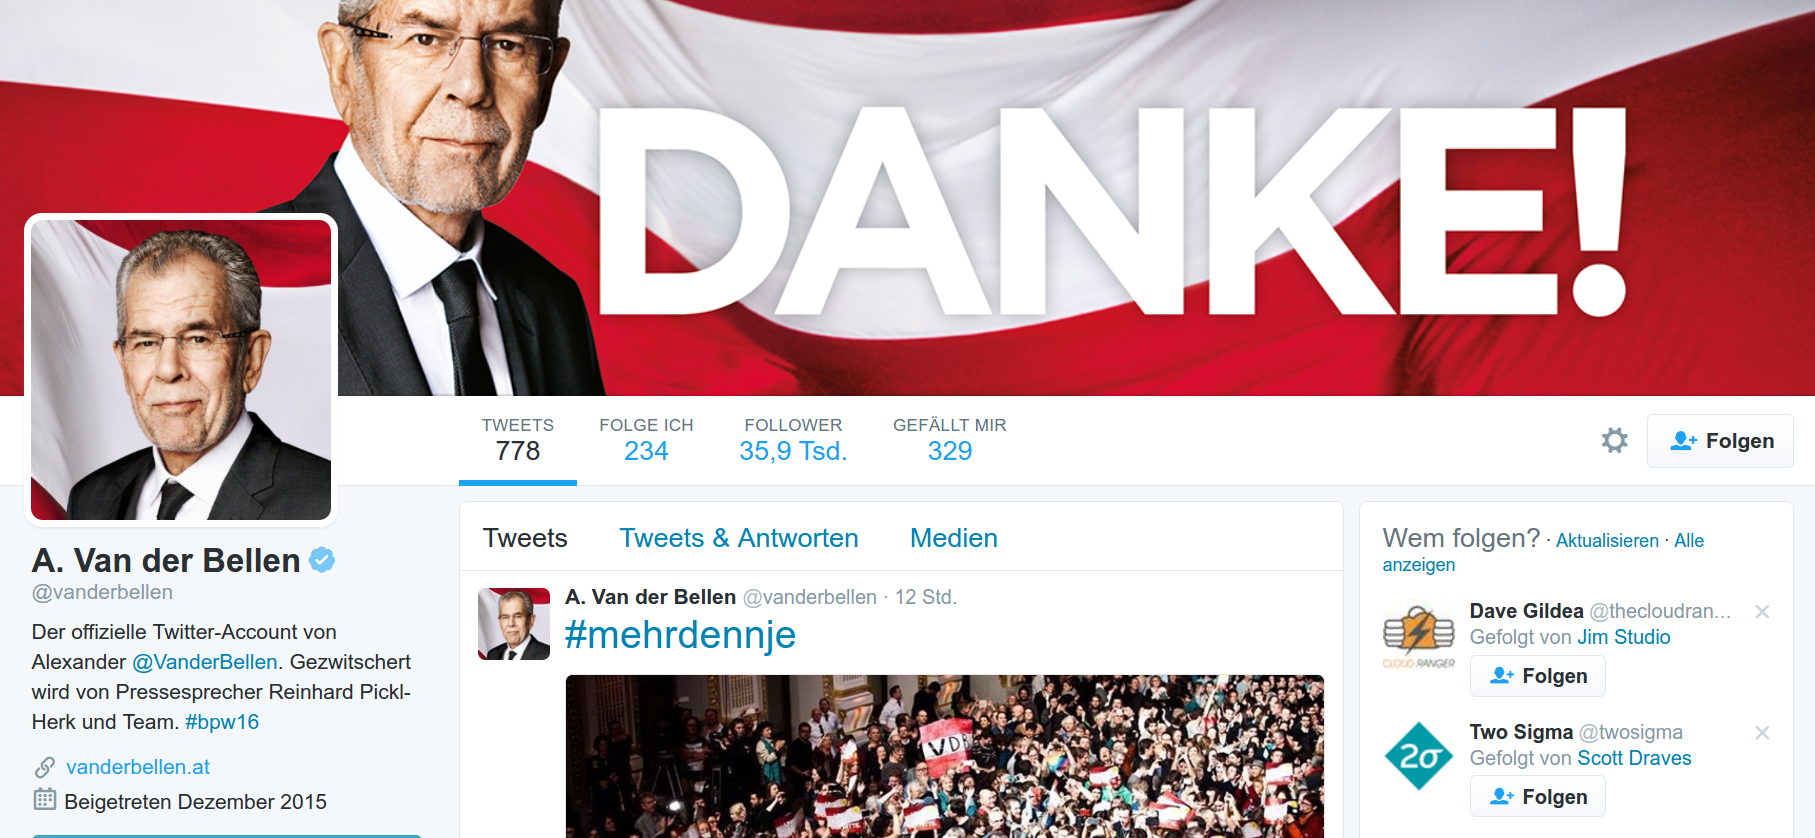
\includegraphics[width=0.7\textwidth]{grafics/vanderbellen_twitter.png}
	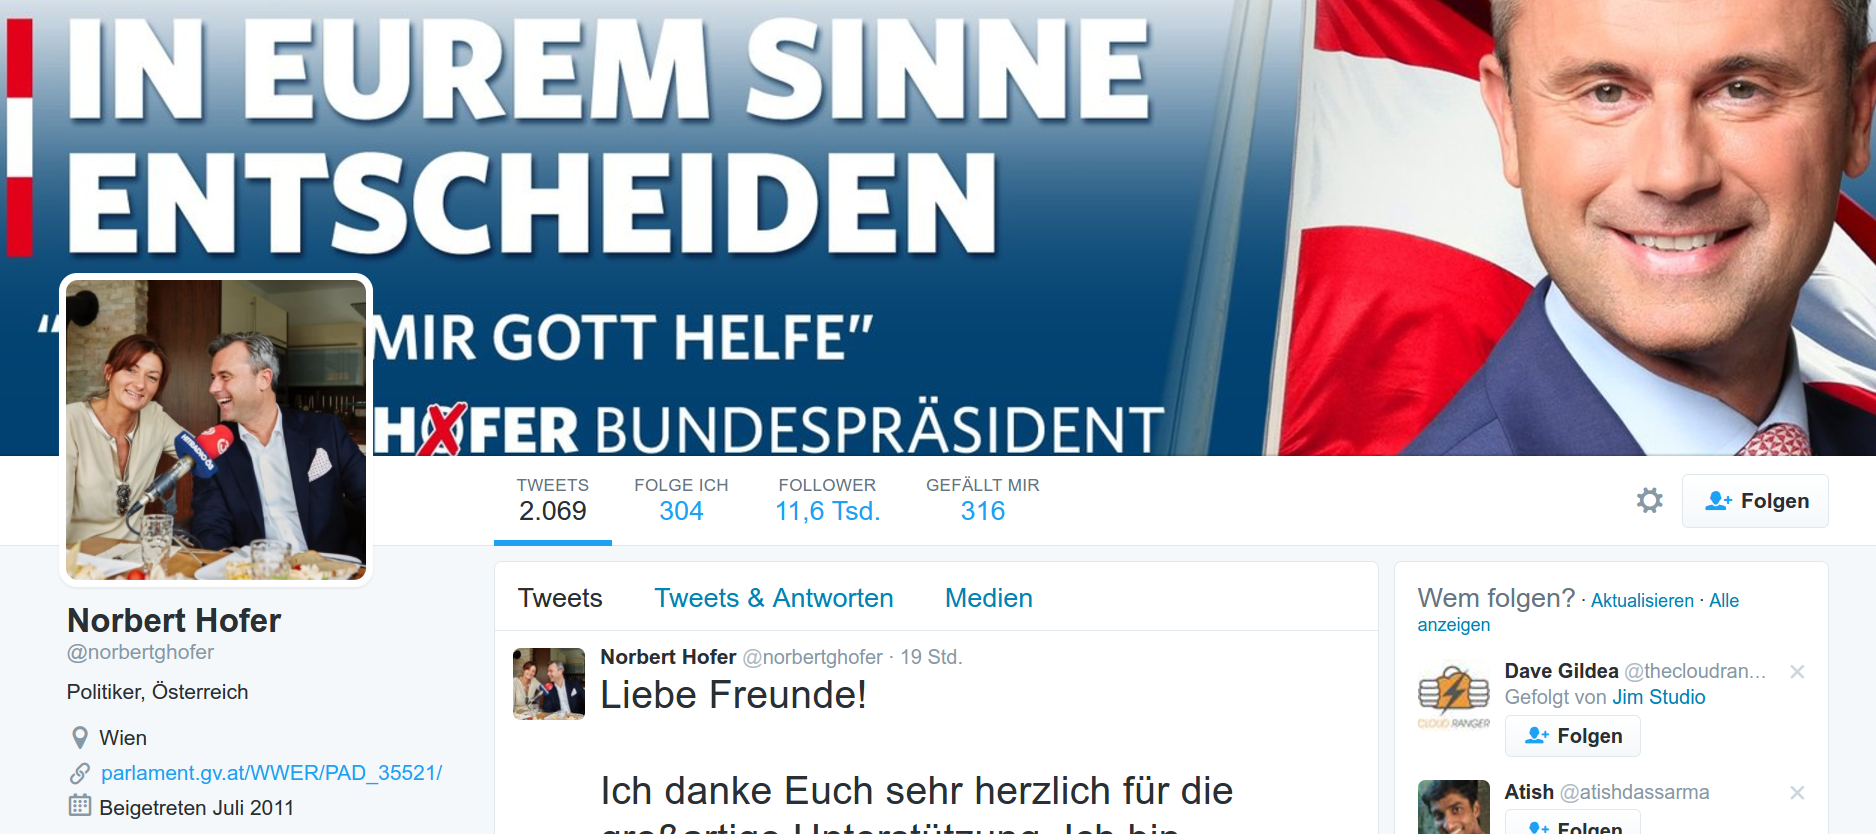
\includegraphics[width=0.7\textwidth]{grafics/hofer_twitter.png} %70% der Textbreite
	\caption{Official twitter account of Norbert Hofer and Alexander Van der Bellen Screencapture right after the election at 04.10.2016}
	\label{fig:Bild1}
\end{figure}

To gather all the tweets of a profile page in an automatic way, twitter offers a REST API\footnote{https://dev.twitter.com/rest/public}. We used this API in conjunction with a small Python script and the Tweepy\footnote{http://www.tweepy.org/} library to generate a dataset for each presidential candidate. When we executed the script one day after the election on October the 5th the script yielded 821 tweets for Alexander Van der Bellen and 2077 tweets for Norbert Hofer.

Our dataset contains the following information for each tweet:
\begin{itemize} 
	\item the 140 character message 
	\item the creation time
	\item how many people have favored the tweet
	\item how many people have retweeted the tweet
	\item if the tweet is a retweet 
	\item the hashtags used in the tweet
	\item the amount of other users mentioned in the tweet
\end{itemize}

To make a comparison possible, we filtered both datasets to only contain tweets from 2016-01-08 to 2016-12-04. The first date is the day Alexander Van der Bellen started his campaign and the second date is, as all Austrians will hopefully know, the election day. This filter left us with 505 tweets for Norbert Hofer and 778 tweets for his opponent. We further excluded retweets. Retweets are tweets of other persons that you can add to your profile page. Retweets show the original favorites and retweets counts and would therefor not be representative of Norbert Hofer's or Alexander Van der Bellen's tweets. Norbert Hofer's dataset contained 90 retweets. Alexander Van der Bellen's dataset contained 117 retweets. This leaves us with 425 tweets for Norbert Hofer and 661 tweets for Alexander Van der Bellen for further analysis. 
\newpage
\section{Analysis}
We already know that Alexander Van der Bellen tweeted more than Norbert Hofer, but we do not know how this tweets are distributed in terms of time. \figurename{2} visualizes the amount of tweets sent per candidate each day from 08.01.2016 to 04.10.2016. Each candidate has one day standing out. Alexander Van der Bellen tweeted 21 times on the 16th of May. This date is six days before the first election which later on got invalidated by the Verfassungsgerichtshof. "Eine Stimme fuer Van der Bellen" was an event in the Wiener Konzerthaus and was held on the 16th of May. The 21 tweets during the day all covered speeches of prominent artists like Andre Heller and pictures of the event.   
\begin{figure}[htbp] 
	\centering
	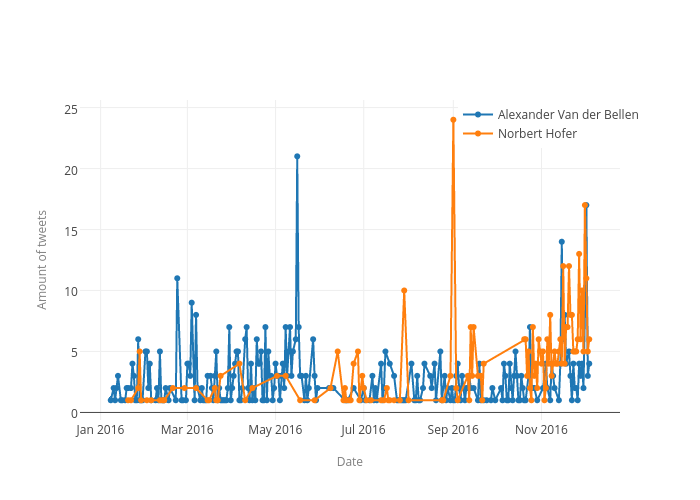
\includegraphics[width=0.8\textwidth]{grafics/tweet_count.png}
	\caption{Amount of Tweets on a daily basis - Norbert Hofer and Alexander Van der Bellen, 08.01.2016 - 04.10.2016}
	\label{fig:Amount of Tweets on a daily basis}
\end{figure}

Norber Hofer tweeted 24 times on the 1st of September. Manually inspecting the tweets revealed that all of them are about hatred in the internet "Hass im Netz". Hofer linked to tweets like: "You are racist. Hitler's Grandson!!" attacking him personally. 

\figurename{2} further shows that Alexander Van der Bellen was more active and more consistent in terms of tweets per day than his opponent. Only during the last two months of the campaign Norbert Hofer started using twitter more often than Alexander Van der Bellen. Before that, Norbert Hofer often did not tweet at all for weeks. Alexander Van der Bellen's tweets are distributed more evenly across all days of the inspected timeframe. 
\newpage
Twitter let's users like tweets. A high number of likes or favorites as it is called in the dataset is a strong indicator for sentiment towards the message contained in the tweet or the person writing the tweet. Norbert Hofer achieved 17.967 favorites, Alexander Van der Bellen 45.974. The mean number of favorites for Alexander Van der Bellen's tweets is approximately 70, for Norbert Hofer it is 42.  \figurename{3} shows the Sum of favorites of all tweets of a day for each day. 
\begin{figure}[htbp] 
	\centering
	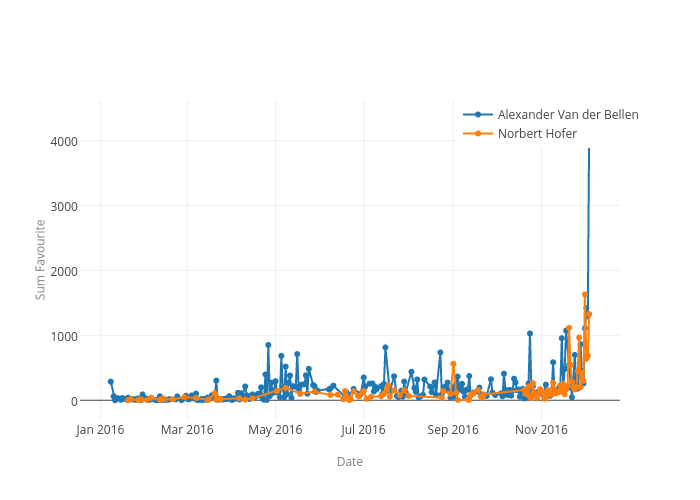
\includegraphics[width=0.8\textwidth]{grafics/favourite.png}
	\caption{Sum of favorite counts on a daily basis - Norbert Hofer and Alexander Van der Bellen, 08.01.2016 - 04.10.2016}
	\label{fig:Sum of favorites on a daily basis}
\end{figure}

It is evident, that tweets from Alexander Van der Bellen were consistently more favored than tweets of his opponent. It is not surprising that the maximum favorites were achieved on election day when the candidates said thank you to all of their supporters. 

It is interesting to note though, that the top favored tweet with a favorite count of 2430 of Alexander Van der Bellen was a thank you tweet on election day using hashtags and a picture. In contrast the top tweet of Norbert Hofer with a favorite count of 431 was a promotion of an interview containing the hashtag\footnote{Hashtags are words prefixed with a \#. They are used in twitter to index topics. Twitter users can search for this topics.} "\#ORFDuell" and a picture. The similarities of hashtag and picture use could indicate that these types of tweets are more successful in terms of getting favored by users than tweets just containing text. Further analysis of this hypothesis is out of scope of this work though.
We furthermore visualized the amount of retweets on a daily basis, but the visualization was similar to \figurename{3} and revealed no further patterns and was therefor omitted from this work.
%\begin{figure}[htbp] 
%	\centering
%	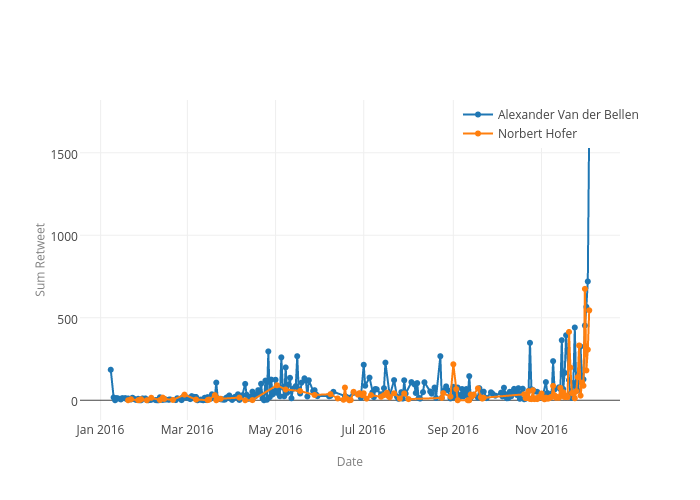
\includegraphics[width=1.0\textwidth]{grafics/retweet.png}
%	\caption{Sum of retweets on a daily basis - Norbert Hofer and Alexander Van der Bellen, 08.01.2016 - 04.10.2016}
%	\label{fig:Sum of retweets on a daily basis}
%\end{figure}
%\newpage
Twitter lets users mention other users with the @ symbol prefixing a username. If a user is mentioned in the tweet, he is notified of the tweet and can react to it. Mentioning a user may foster direct conversation on specific topics. 

Alexander Van der Bellen has mentioned other users 257 times. Norbert Hofer' tweets contain other users 84 times.  

\begin{figure}[htbp] 
	\centering
	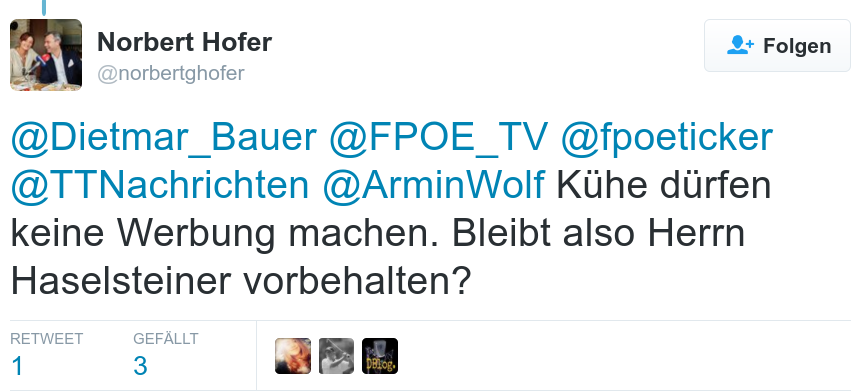
\includegraphics[width=0.6\textwidth]{grafics/most_mentioned_hofer.png}
	\caption{Norbert Hofer's tweet mentioning 5 other users}
	\label{fig:Norbert Hofer most mentioned}
\end{figure}
\begin{figure}[htbp] 
	\centering
	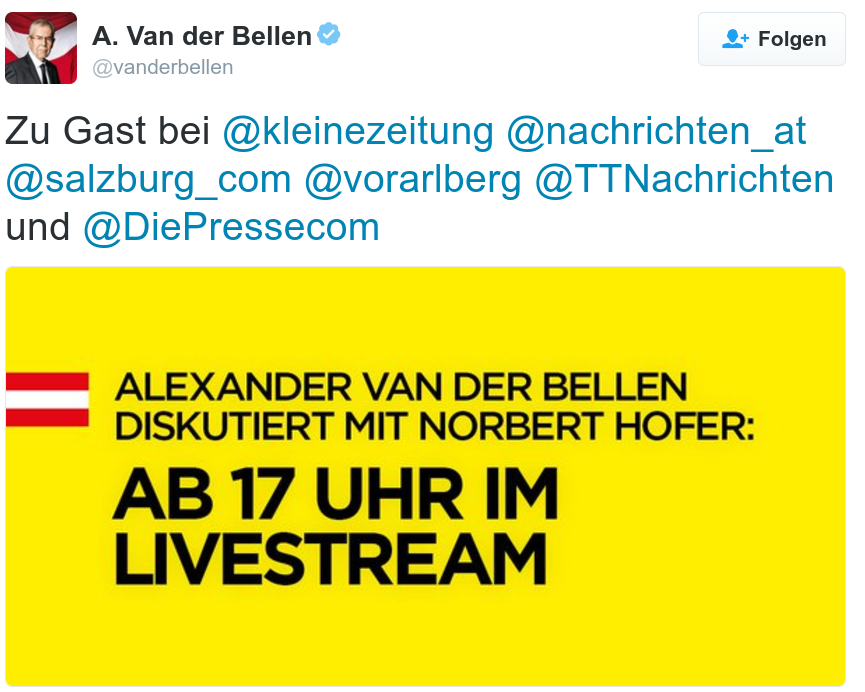
\includegraphics[width=0.6\textwidth]{grafics/most_mentioned_vdb.png}
	\caption{Alexander Van der Bellen's tweet mentioning 6 other users}
	\label{fig:Norbert Hofer most mentioned}
\end{figure}

\figurename{4} and \figurename{5} show Norbert Hofer's and Alexander Van der Bellen's tweets containing the maximum amount of other users mentioned. Alexander Van der Bellen is promoting a live stream and Norbert Hofer's intention is not clearly evident for us because of missing contextual information.

%\begin{figure}[htbp] 
%	\centering
%	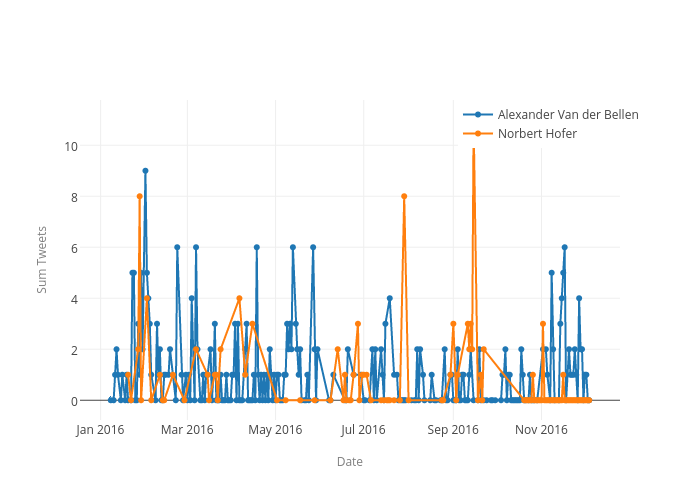
\includegraphics[width=0.8\textwidth]{grafics/user_mention.png}
%	\caption{Sum of user mentioned - Norbert Hofer and Alexander Van der Bellen, 08.01.2016 - 04.10.2016}
%	\label{fig:Sum of retweets on a daily basis}
%\end{figure}

\section{Topics}
In the previous chapter we analyzed the gathered tweets regarding amount, topology, favorites received, other users mentioned and hashtags used. In this part we try to find out what the main topics used by the candidates were. We employ word clouds to shine light on this question. A word cloud visualized the words used in a text corpus. The font size of each word represents the amount of times the word is used in the corpus. Often used words are bigger than less often used words therefor giving an indication of importance. \figurename{6} and \figurename{7} show the word clouds for Norbert Hofer's and Alexander Van der Bellens tweets after we removed german stop words such as "wer, wie , und,..". \figurename{8} and \figurename{9} visualize the hashtags used by both candidates.
\begin{figure}[htbp] 
	\centering
	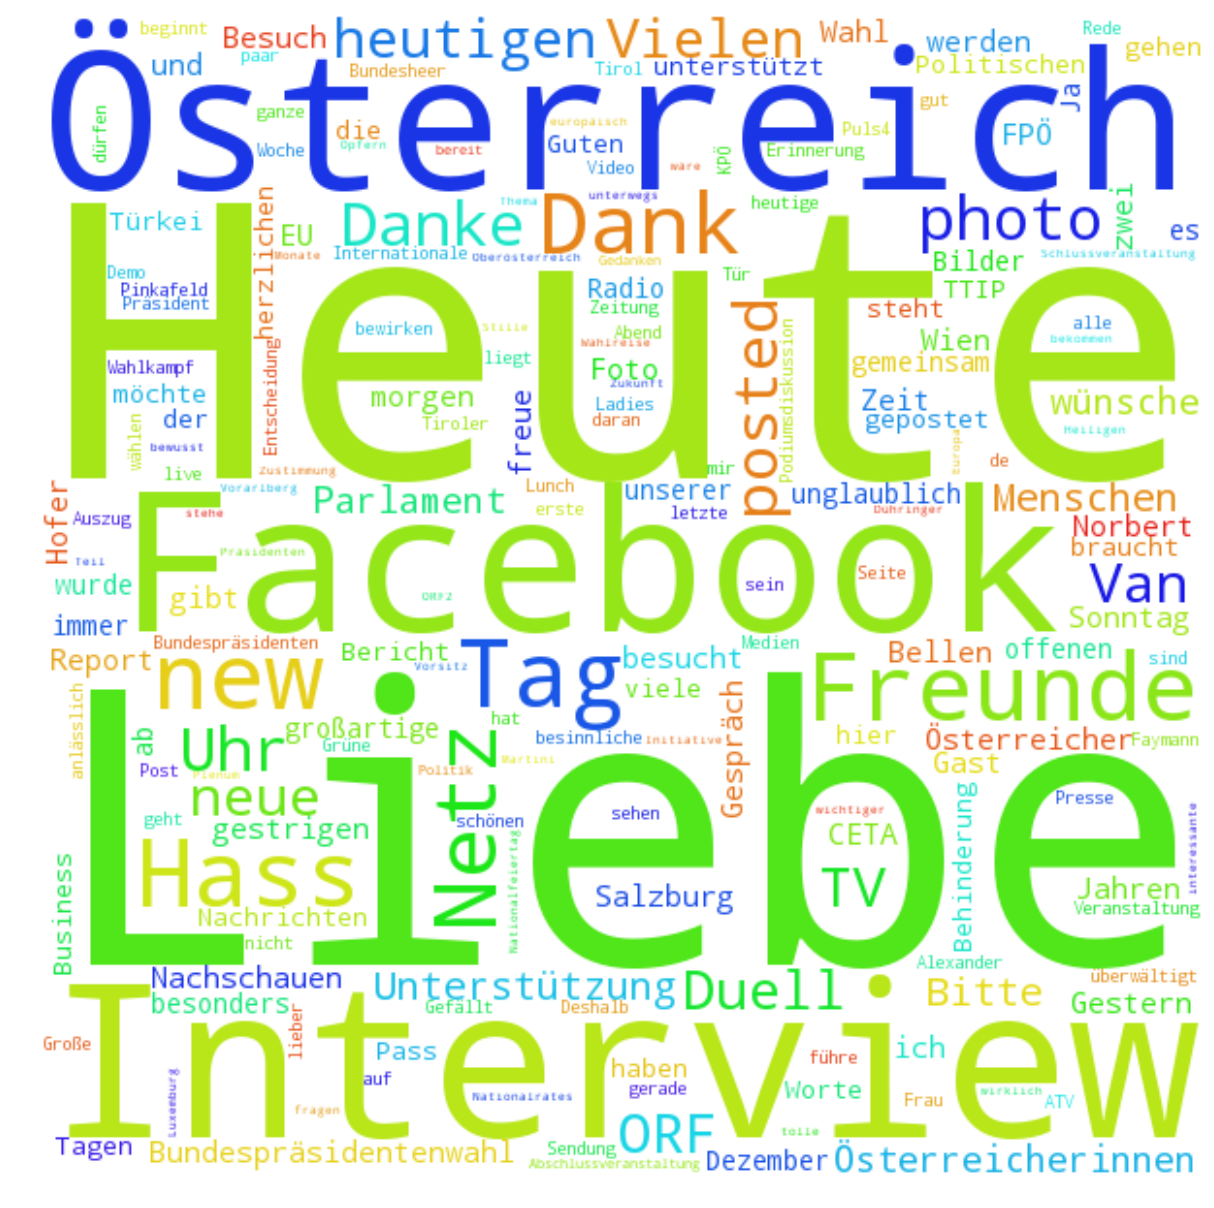
\includegraphics[width=0.8\textwidth]{grafics/wordcloud_hofer.png}
	\caption{Wordcloud Norbert Hofer, Tweets from 08.01.2016 - 04.10.2016}
	\label{fig:Wordcloud Norbert Hofer}
\end{figure}
\newpage
\begin{figure}[htbp] 
	\centering
	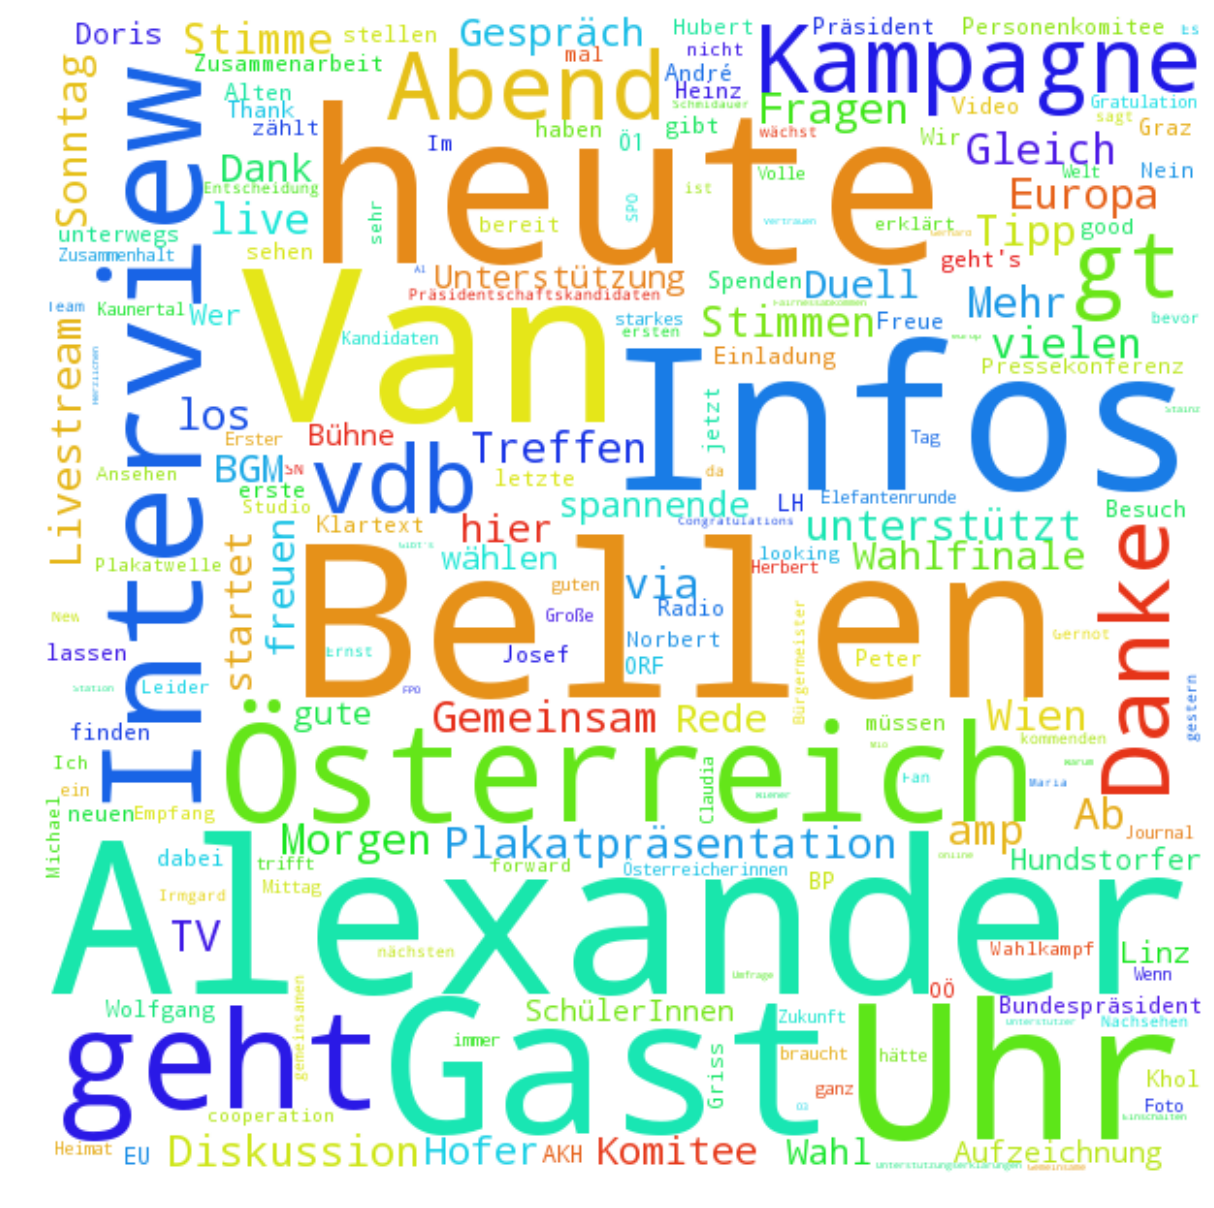
\includegraphics[width=0.8\textwidth]{grafics/wordcloud_vdb.png}
	\caption{Wordcloud Alexander Van der Bellen, Tweets from 08.01.2016 - 04.10.2016}
	\label{fig:Wordcloud Alexander Van der Bellen}
\end{figure}
Both presidential candidates use words related to events and rallies very often. Example words for this category are:"Interview", "Infos", "Orf", "Gast", "Diskussion", "Livestream", "Duell", "Heute" and "Kampagne". Norbert Hofer used very emotional words like "Liebe" and "Hass". Furthermore he emphasized on Facebook, linking to videos and content uploaded there. In contrast Alexander Van der Bellen included his name in a prominent way. Both candidates convey strong political opinions on specific topics such as the European Union, immigration and the labor market which can be found on their personal pages \footnote{Alexander Van der Bellen: https://www.vanderbellen.at/ziele-inhalte/; Norbert Hofer: https://www.norberthofer.at/ Positionen}. Alexander Van der Bellen's word cloud only contains the word Europe and Norbert Hofer's only topical keyword present in the word cloud is TTIP. This leads us to the conclusion that both candidates are simply broadcasting their messages and were not discussing with the public about specific political topics.
\newpage
\begin{figure}[htbp] 
	\centering
	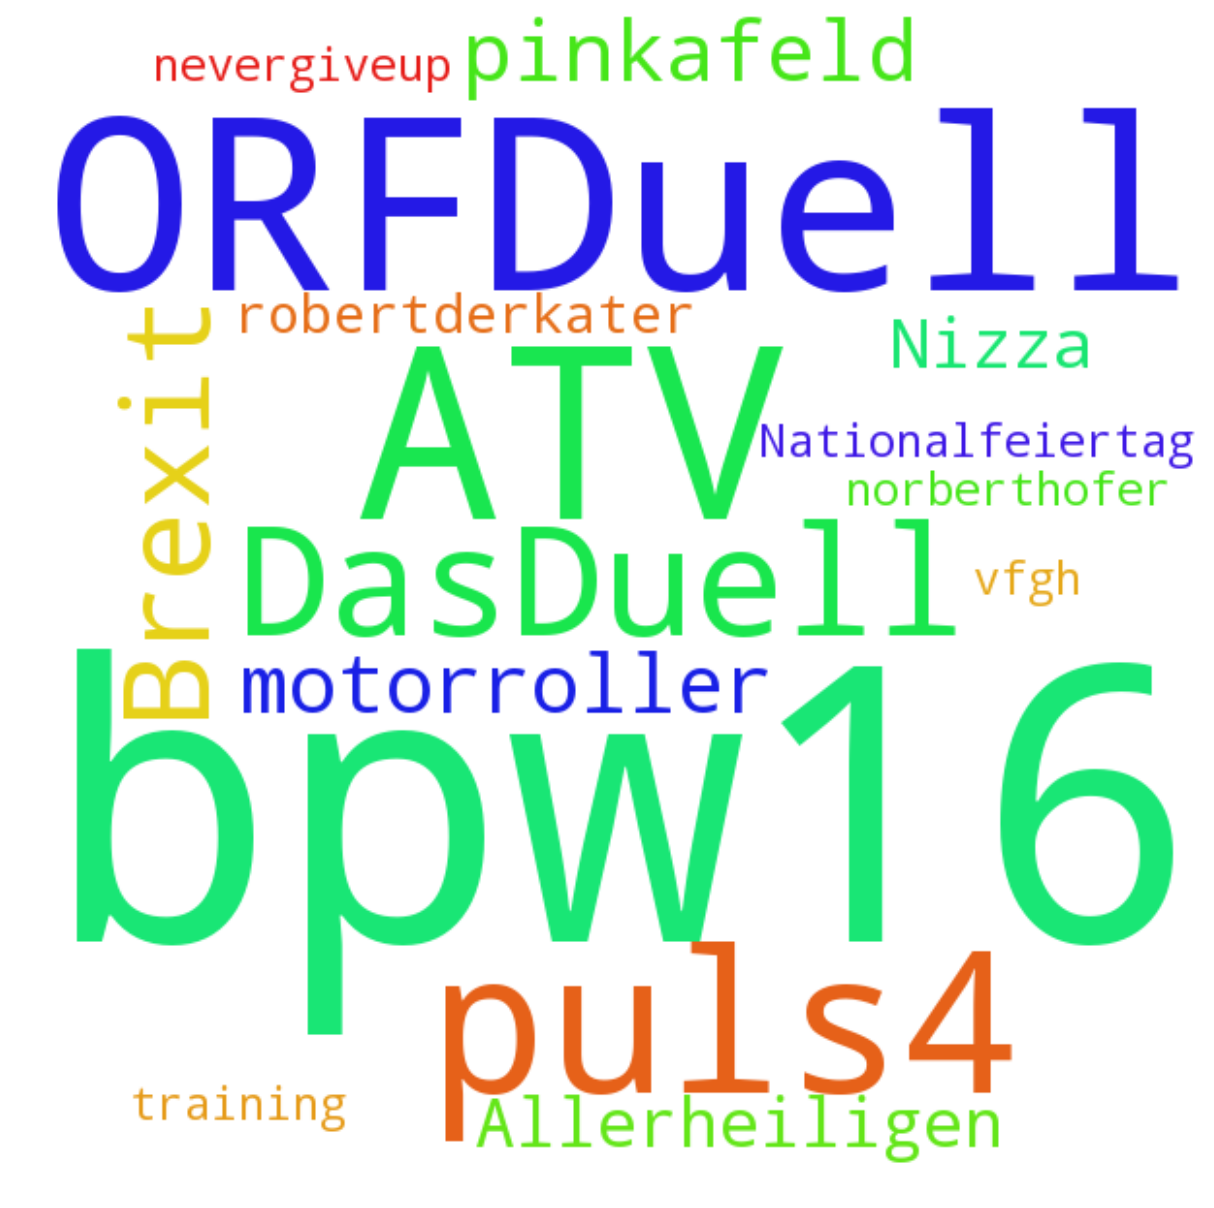
\includegraphics[width=0.7\textwidth]{grafics/wordcloud_hofer_hashtags.png}
	\caption{Hashtag Wordcloud Norbert Hofer, Tweets from 08.01.2016 - 04.10.2016}
	\label{fig:Wordcloud Norbert Hofer Hashtags}
\end{figure}
\begin{figure}[htbp] 
	\centering
	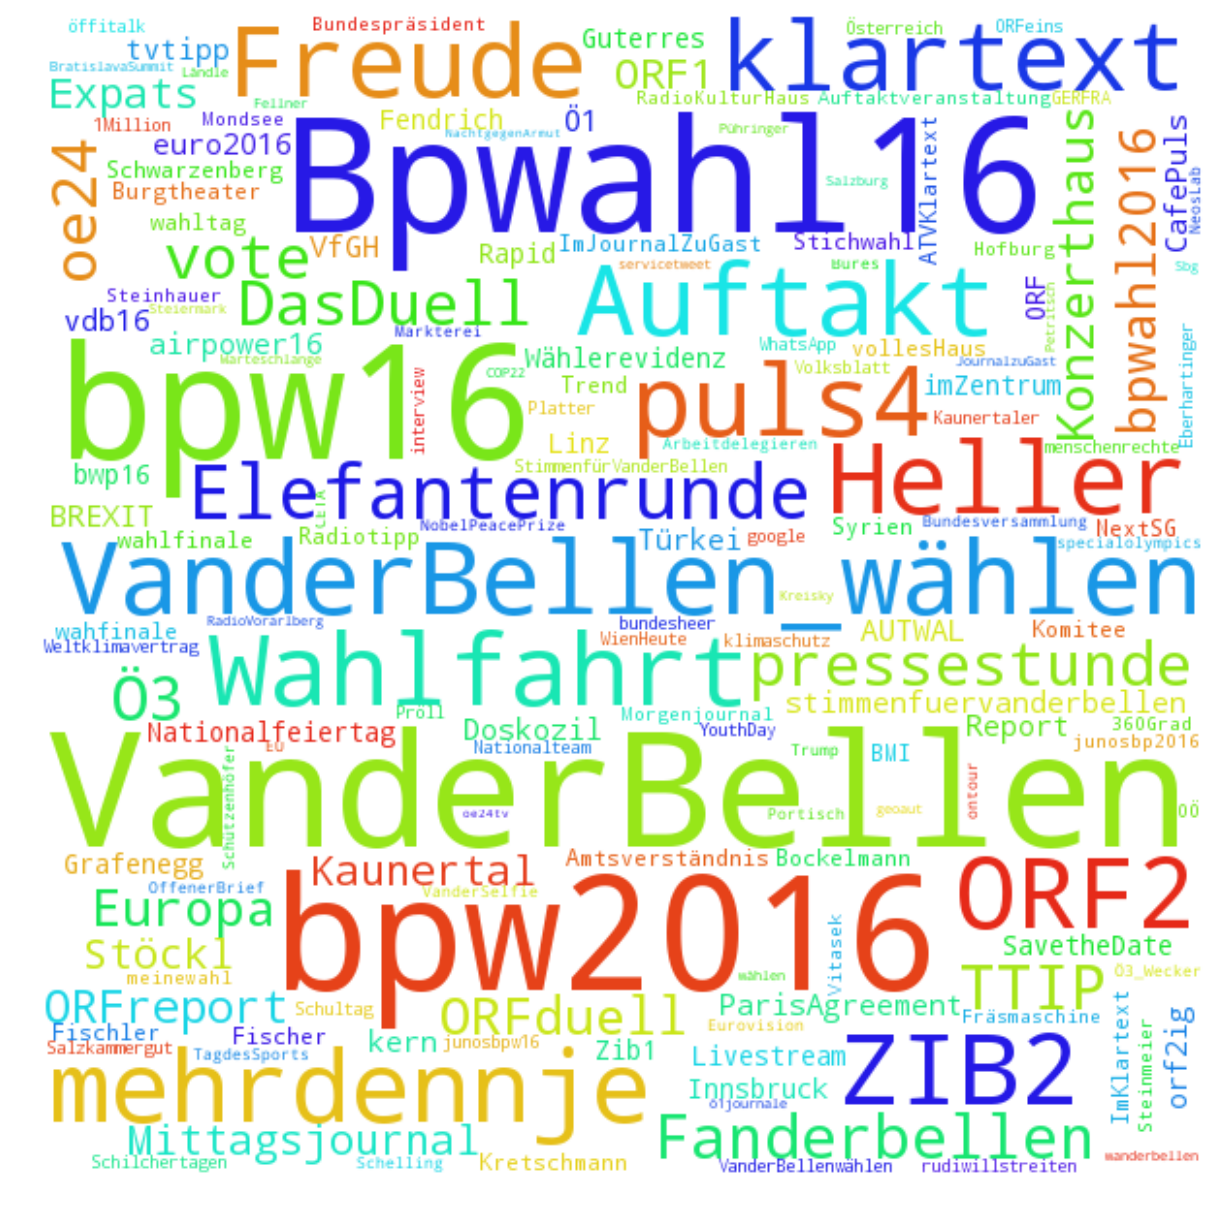
\includegraphics[width=0.7\textwidth]{grafics/wordcloud_vdb_hashtags.png}
	\caption{Hashtag Wordcloud Alexander Van der Bellen, Tweets from 08.01.2016 - 04.10.2016}
	\label{fig:Wordcloud Alexander Van der Bellen Hashtags}
\end{figure}
It is evident that Norbert Hofer's use of hashtags is way less prominent than Alexander Van der Bellen's. Both candidates use hashtags defining the election itself such as "bpw16", "bpw2016" and "bpwahl16". Again political topics are mostly missing. Alexander Van der Bellen uses hashtags for specific events such as "pressestunde", "konzerthaus" and "wahlfahrt" makes his tweets more easily searchable for interested citiziens. We have no real explanation for the use of the hashtag "robertderkater" of Norbert Hofer apart from giving his cat a platform and making him look more human and animal loving. 
\newpage
\section{Discussion and Future Work}
In this work we presented descriptive analysis and word cloud visualizations of both candidates of the 2016 presidential election which was won by Alexander Van der Bellen, therefor giving much needed insights into social media use during Austrian elections. 
We showed that Alexander Van der Bellen was more active and could generate more reactions and likes than his opponent. Furthermore we showed that Both candidates mainly used twitter to broadcast their message and inform about upcoming events such as television shows or rallies and did not engange in discussion about political topics such as immigration or labor market issues.
Since we have no data on individual voters and how they are represented on twitter, we cannot say if the use of social media has influenced election results. However we see the victory of Alexander Van der Bellen in the election in relation his overwhelming success on twitter during the campaign as a sign that there may be at least correlation. In future research we would like to study the correlation between the election results and social media engagement of the candidates. 
We would be further interested in analyzing the users who favored either candidates tweets. Are there age, gender, social stratum differences in users who like and follow either candidate?
Moreover it would be interesting to classify the tweets into different classes like information tweet with hashtag and picture, or politicial topic tweet, or reaction mentioning different users and analyze which classes are more favored by users.



%
% ---- Bibliography ----
%
\begin{thebibliography}{5}
%
\bibitem{aaker2010obama}
Jennifer Aaker and Victoria Chang.
\newblock Obama and the power of social media and technology.
\newblock {\em The European Business Review}, pages 17--21, 2010.

\bibitem{effing2011social}
Robin Effing, Jos van Hillegersberg, and Theo Huibers.
\newblock Social media and political participation: are facebook, twitter and
youtube democratizing our political systems?
\newblock In {\em International Conference on Electronic Participation}, pages
25--35. Springer, 2011.

\bibitem{graham2013between}
Todd Graham, Marcel Broersma, Karin Hazelhoff, and Guido van't Haar.
\newblock Between broadcasting political messages and interacting with voters:
The use of twitter during the 2010 uk general election campaign.
\newblock {\em Information, Communication \& Society}, 16(5):692--716, 2013.

\bibitem{larsson2012studying}
Anders~Olof Larsson and Hallvard Moe.
\newblock Studying political microblogging: Twitter users in the 2010 swedish
election campaign.
\newblock {\em New Media \& Society}, 14(5):729--747, 2012.

\bibitem{miller2015studying}
Noah~W Miller and Rosa~S Ko.
\newblock Studying political microblogging: Parliamentary candidates on twitter
during the february 2012 election in kuwait.
\newblock {\em International Journal of Communication}, 9:21, 2015.

\bibitem{tumasjan2010predicting}
Andranik Tumasjan, Timm~Oliver Sprenger, Philipp~G Sandner, and Isabell~M
Welpe.
\newblock Predicting elections with twitter: What 140 characters reveal about
political sentiment.
\newblock {\em ICWSM}, 10:178--185, 2010.



\end{thebibliography}

\clearpage
\addtocmark[2]{Author Index} % additional numbered TOC entry
\renewcommand{\indexname}{Author Index}
\printindex
\clearpage
\end{document}
